\documentclass{article}
\usepackage[utf8]{inputenc}
\usepackage[left=1.50cm, right=1.50cm, top=1.50cm, bottom=1.50cm]{geometry}
\usepackage{blindtext}
\usepackage{multicol}
\usepackage{graphicx}
\usepackage{listings}
\usepackage{xcolor}

\title{Ordenamiento burbuja}
\author{Gustavo Ramos}
\date{7 de Enero 2024}

\definecolor{codegreen}{rgb}{0,0.6,0}
\definecolor{codegray}{rgb}{0.5,0.5,0.5}
\definecolor{codepurple}{rgb}{0.58,0,0.82}
\definecolor{backcolour}{rgb}{0.95,0.95,0.92}

\lstdefinestyle{mystyle} {
	backgroundcolor=\color{backcolour},   
	commentstyle=\color{codegreen},
	keywordstyle=\color{magenta},
	numberstyle=\tiny\color{codegray},
	stringstyle=\color{codepurple},
	basicstyle=\ttfamily\footnotesize,
	breakatwhitespace=false,         
	breaklines=true,                 
	captionpos=b,                    
	keepspaces=true,                 
	numbers=left,                    
	numbersep=5pt,                  
	showspaces=false,                
	showstringspaces=false,
	showtabs=false,                  
	tabsize=2
}

\lstset{style=mystyle}

\begin{document}
	
	\maketitle
	\begin{multicols}{2}
		
		\section{Resumen}
		La practica siguiente expone el algoritmo burbuja para ordenar números y su comprensión para poderlo programar en el lenguaje c.
		
		\section{Introducción}
		Los arrays son la contraparte computacional de los vectores y las matrices, los mas simples son los arrays que se asemejan a vectores de n-dimensión, los arrays en la programación suelen representarse como Var[n], donde Var es el nombre y n es la dimensión del mismo, estos suelen iniciar en la componte 0, eso quiere decir, que Var[I] puede almacenar I+1 valores en un espacio en la memoria física de nuestra computadora.
		En el caso para c, la estructura de un array suele ser de la forma -tipo Var[I];-, donde en tipo se asigna el tipo de variable (double, char, float, int, etc.)
		
		
		\section{Marco teórico }
		El ordenamiento burbuja es un algoritmo que ordena números comparando dos entre si, al tener n elementos, el algoritmo encierra los dos primero números en una burbuja y los compara, si el segundo numero es menor al primero, entonces los intercambia de lugar, si no, los deja igual, sigue comparando el segundo número con el tercero y repite hasta el n-1 número y el n número, compara una segunda vez, una tercera una cuarta y hasta una $(n^2-2)/2$ cantidad de comparaciones, esto se consigue gracias a dos bucles que accederán a los números en diferente orden y esto lo conseguirán gracias a una sentencia if para comparar ambos números.
		
		
		
	\end{multicols}
	
	\section{Diseño de código }
	
	\lstinputlisting[language=c]{../Burbuja.c}
	\newpage
	
	\begin{multicols}{2}
		
		\section{Análisis  de resultados}
		Podemos ver dos ejemplos del código funcionando perfectamente:
		\begin{center}
			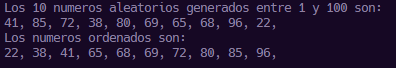
\includegraphics[scale=0.8]{1.png} \\
		\end{center}
		\begin{center}	
			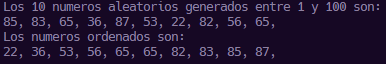
\includegraphics[scale=0.82]{2.png}
		\end{center}
		
		\section{Conclusiones}
		El ordenamiento de burbuja es el algoritmo mas sencillo para ordenar números, y así mismo, elementos a los que les podamos asignar un numero, programarlo es muy sencillo, sin embargo, su eficiencia computacional no lo es tanto.
		La generación de los números aleatorios es interesante y deja en claro que nuestro programa funciona, puesto que nosotros no conocemos dichos números y tampoco somos capaces de manipularnos a nuestro antojo para ordenarlos de manera "manual", sino solo a través del algoritmo.
		
		\section{Referencias }
		[1] Astrachan, Owen (2003). Ordenamiento de burbuja: Un análisis arqueológico de un algoritmo
	\end{multicols}
	
	
\end{document}